
\subsection*{5.2 Measures of Central Tendency}
Measures of central tendency describe the center of a data set using three main statistics: mean, median, and mode.

\textbf{Key Concepts:}

\begin{itemize}
	\item \textbf{Mean:} The arithmetic average of a data set, calculated as:
	\[
	\text{Mean} = \frac{\sum x f}{\sum f},
	\]
	where $x$ represents the class midpoint, and $f$ is the frequency.\\
	In case of grouped data use midpoints of each group to estimate the mean (see Example 2.)
	
	\item \textbf{Median:} The middle value in an ordered data set. Note that the data must be ordered first. \\
	\begin{itemize}
		\item For an odd number of values: The median is the middle number. \\
		Example: Data = $1,2,3,4,5$ \\ Median = $3$.
		\item For an even number of values: The median is the average of the two middle numbers. \\
		Example: Data = $1,2,3,4,5,6$ \\ Median = $\frac{3+4}{2} = 3.5$.
	\end{itemize}
	
	\item \textbf{Mode:} The most frequently occurring value in a dataset. For grouped data, the modal class is the class with the highest frequency. 
	
	\begin{itemize}
		\item If a number appears most frequently, it is the mode. \\
		Example: Data = $1,2,2,3,2,4,5,6,4,3,2,3,4,2,3,2,6,5$ \\
		Frequency: 
		\begin{itemize}
			\item $1$ appears once.
			\item $2$ appears \textbf{6} times.
			\item $3$ appears 5 times.
			\item $4$ appears 3 times.
			\item $5$ appears 2 times.
			\item $6$ appears 2 times.
		\end{itemize}
		Mode = \textbf{2} (most frequent value).
	\end{itemize}
	
	\item \textbf{Graph work:} You can find certain measures of central tendency from cumulative frequency graph or histograms. See examples 3 and 4 for details.
\end{itemize}

\textbf{Examples:}

\begin{flushleft}
	\textbf{Example 1: Find the Mean, Median, and Mode of the Given Data Set.}
	
	\textbf{Given Data:} \\ 
	$12, 7, 10, 15, 10, 18, 12, 10, 14, 7, 16, 12, 10, 9, 10$
	
	\vspace{0.5cm}
	\textbf{Solution:}
	
	\textbf{Step 1: Find the Mode}
	\begin{itemize}
		\item Count the frequency of each number:
		\begin{itemize}
			\item $7$ appears twice.
			\item $9$ appears once.
			\item $10$ appears \textbf{5} times.
			\item $12$ appears 3 times.
			\item $14$ appears once.
			\item $15$ appears once.
			\item $16$ appears once.
			\item $18$ appears once.
		\end{itemize}
		\item The mode is the number that appears most frequently.
		\[
		\text{Mode} = 10
		\]
	\end{itemize}
\end{flushleft}

\textbf{Step 2: Find the Median}
\begin{itemize}
	\item Arrange the data in ascending order:
	\[
	7, 7, 9, 10, 10, 10, 10, 10, 12, 12, 12, 14, 15, 16, 18
	\]
	\item Find the middle value. Since there are 15 numbers (odd count), the median is the 8th value.
	\[
	\text{Median} = 10
	\]
\end{itemize}

\textbf{Step 3: Find the Mean}
\begin{itemize}
	
	\item Use the mean formula:
	\[
	\text{Mean} = \frac{\sum x}{n}
	\]
	\item Calculate the sum of all numbers:
	\[
	7 + 7 + 9 + 10 + 10 + 10 + 10 + 10 + 12 + 12 + 12 + 14 + 15 + 16 + 18 = 162
	\]
	
	\item Divide by the total number of values ($n=15$):
	
\end{itemize}

\begin{flushleft}
	\textbf{Example 2: Find the mean from the following frequency distribution.}
	
	\begin{center}
		\begin{tabular}{c|c|c}
			\textbf{Class Interval} & \textbf{Frequency (f)} & \textbf{Midpoint (x)} \\
			\hline
			0 - 10 & 4 & 5 \\
			10 - 20 & 6 & 15 \\
			20 - 30 & 8 & 25 \\
			30 - 40 & 10 & 35 \\
			40 - 50 & 7 & 45 \\
		\end{tabular}
	\end{center}
	
	\vspace{0.5cm}
	\textbf{Solution:}
	\vspace{0.5cm}
	
	Using the formula:
	\[
	\text{Mean} = \frac{\sum x f}{\sum f}.
	\]
	
	\[
	\text{Mean} = \frac{(5 \times 4) + (15 \times 6) + (25 \times 8) + (35 \times 10) + (45 \times 7)}{4 + 6 + 8 + 10 + 7}.
	\]
	
	\[
	= \frac{20 + 90 + 200 + 350 + 315}{35}.
	\]
	
	\[
	= \frac{975}{35} = 27.86.
	\]
	
	Thus, the mean is approximately $27.86$.
\end{flushleft}

\begin{flushleft}
	\textbf{Example 3: Determine the median from the cumulative frequency curve (ogive) below.}
	
	\vspace{0.5cm}
	
	\begin{center}
		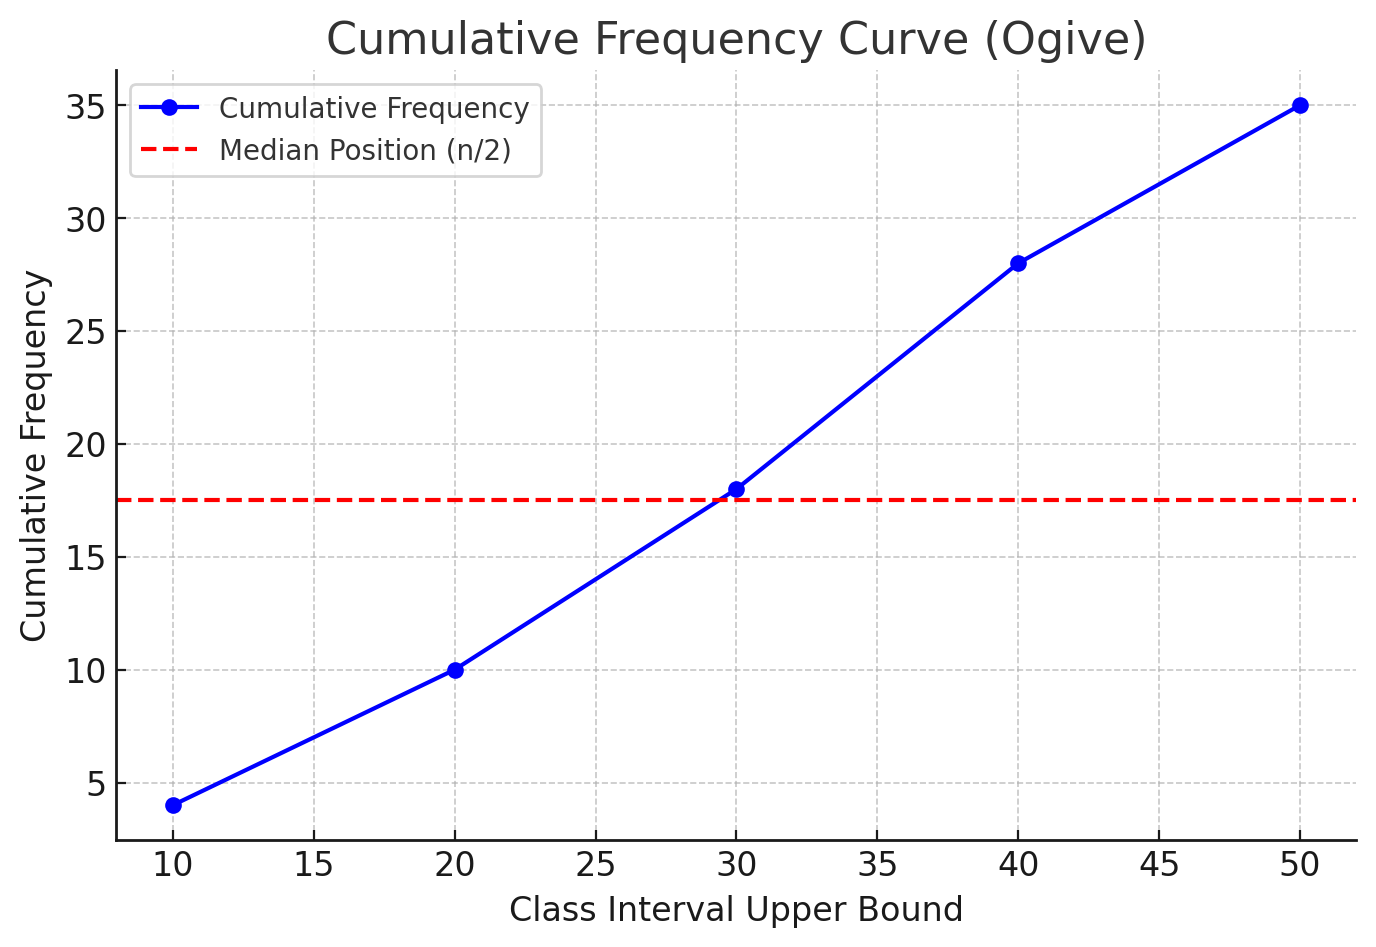
\includegraphics[width=0.6\textwidth]{5.4.png}
		\captionof{figure}{Cumulative Frequency Curve (Ogive)}
	\end{center}
	
	\vspace{0.5cm}
	\textbf{Solution:}
	\vspace{0.5cm}
	
	Step 1: Identify the total number of observations $n$.
	
	Step 2: Find the median position: $\frac{n}{2} = \frac{35}{2}=17.5$.
	
	Step 3: Locate the corresponding value on the cumulative frequency curve: dashed red line on the graph.
	
	Step 4: Use interpolation if necessary to estimate the median value.
	Solution is the intersection of cummulative frequency curve and dashed line.
	From the graph, the estimated median is around $28$.
\end{flushleft}
\begin{flushleft}
	\textbf{Example 4: Determine the Mode from the Given Histogram.}
	\begin{center}
		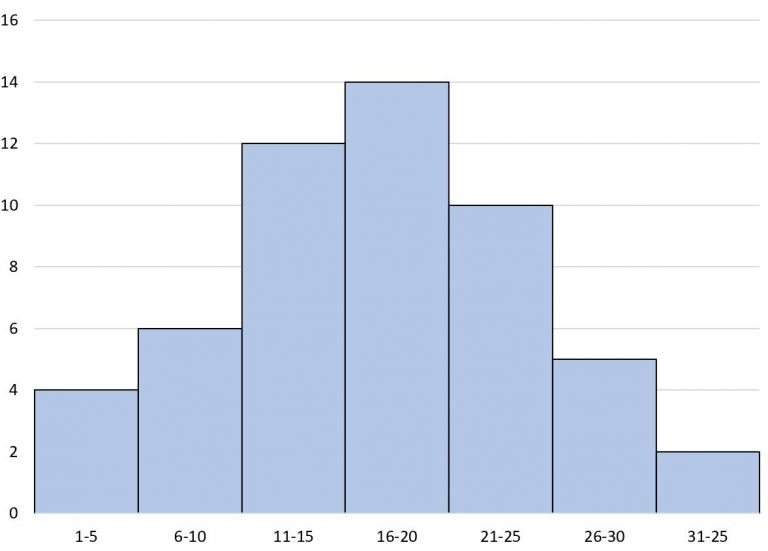
\includegraphics[width=0.7\textwidth]{5.7.jpg}
		
	\end{center}
	
	\textbf{Solution:}
	
	Step 1: Identify the modal class.
	\begin{itemize}
		\item The modal class is the class interval with the highest frequency, which is $16-20$.
	\end{itemize}
	
	Step 2: Use the histogram and the line intersection method.
	\begin{itemize}
		\item Draw two diagonal lines from the tops of the bars adjacent to the modal class, forming an "X" shape.
		\begin{center}
			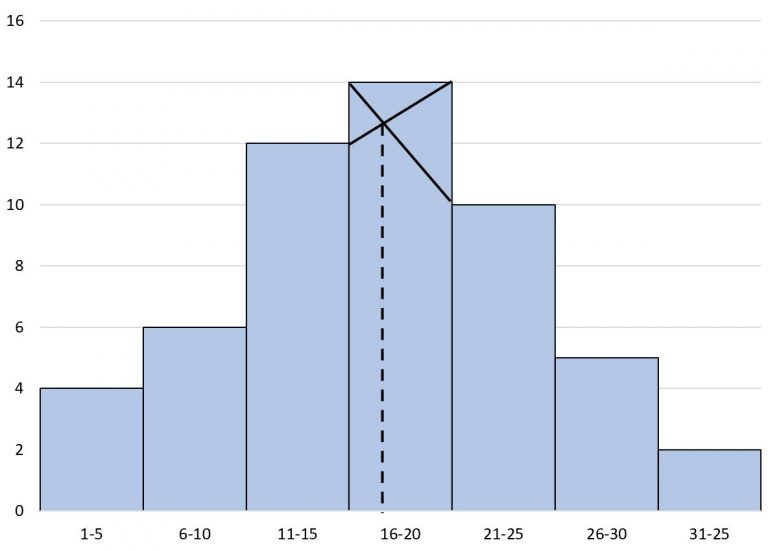
\includegraphics[width=0.7\textwidth]{5.6.jpg}
			\captionof{figure}{Histogram with Mode Estimation Using Line Intersection.}
		\end{center}
		\item The intersection of these lines falls near $x \approx 17$, which represents the estimated mode.
	\end{itemize}
	
	Step 3: Conclusion.
	\begin{itemize}
		\item From the visual estimation, the mode is approximately:
		\[
		\textbf{Mode} \approx 17.
		\]
	\end{itemize}
	
	\vspace{0.5cm}
	
	
	Thus, the mode is visually estimated to be around 17.
\end{flushleft}
